 %%%%%%%%%%%%%%%%%%%%%%%%% CHAPTER %%%%%%%%%%%%%%%%%%%%%%%%%%%%%%%%
\chapter{Introducción a las redes neuronales convolucionales}


La literatura de las redes neuronales data desde \textcolor{red}{inserte fecha}. Sin embargo, no fue hasta el \textcolor{red}{2015} con la introducción de las \textsl{redes neuronales convolucionales} (CNN por sus siglas en inglés) \textcolor{blue}{que la comunidad científica empezó a prestar especial atención}. Para entender a profundidad a las CNNs, definiremos lo que es una convolución. Para un estudio más detallado es posible consultar \cite{CNNdefinition,deeplearningbook}. 

%------------------------------ 1.Convoluciones -----------------------
\section{Convoluciones}
En matemáticas, se suele referir a la convolución de dos funciones $f$ y $g$.
 \begin{definition}[Convolución]
     Sean $f,g : \R \to \R$. La convolución de $f$ con $g$, denotada como $f * g$ se define como:
     $$(f*g)(t) = \int_{0}^t f(\tau)g(t-\tau)d\tau$$
 \end{definition}
 Ésta definición sin embargo no es muy práctica para los paradigmas computacionales, pues  las limitaciones físicas nos obligan a traducir la integral como una \textcolor{red}{suma de intervalos muy pequeños}. Además, si tomamos $f$ como una imagen, es necesario considerar más de una dimensión.
 \begin{definition}[Convolución de una imagen con un kernel]
     Sea $I$ una imagen y $K$ un kernel bidimensional. La convolución de $I$ con $K$ es la imagen $(I*K)$ definida como:
     $$(I*K)(i,j) = \sum_m\sum_n I(m,n)K(i-m,j-n).$$ 
 \end{definition}
 En varias librerías de aprendizaje automático se implementa una correlación cruzada en lugar de una convolución. La única diferencia entre una correlación cruzada y una convolución es la orientación del Kernel. En este trabajo, adoptaremos la convención usual de referirnos a las correlaciones como convoluciones.
 \begin{definition}
     Sea $I$ una imagen y $K$ un kernel bidimensional. La correlación cruzada de $I$ con $K$ es la imagen definida por 
     $$(I*K)(i,j) = \sum_m\sum_n I(i+m,j+n)K(m,n).$$ 
 \end{definition} 

 \begin{figure}[H]
     \centering
     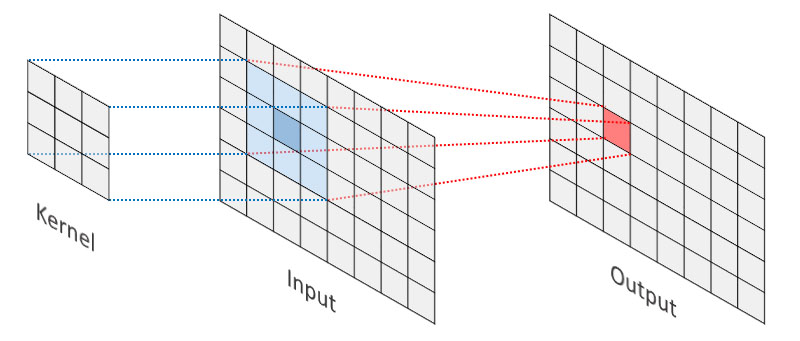
\includegraphics[width=4in]{../src/ch1convolution.jpg}
     \caption{\textsc{Representación gráfica de una convolución. Para cada posición del Kernel sobre la imagen, se realiza una multiplicación \textsl{entrada por entrada} del Kernel y la un conjunto de pixeles de la imagen, del mismo tamaño que el Kernel.}} 
 \end{figure}
 Cuando calculamos nuestra correlación cruzada, desplazamos el kenrel 1 pixel a la vez. Sin embargo, es posible aumentar la cantidad de pixeles que avanza el kernel en cada iteración. A esto se le conoce como tamaño de paso
 %------------------------------ Stride -----------------------
 \subsection{Stride}
 \begin{definition}
    Sea $x$ una característica, y $K$ un kernel. Denotamos la correlación cruzada con tamaño de paso $a$ como 
    \begin{equation}
        \textcolor{red}{(I*K)|_a = (I*K)(i,j) = \sum_m\sum_n I(i+m+a*i,j+n+a*j)K(m,n)}
    \end{equation}
 \end{definition}
 Debido a nuestras convenciones en la notación, a la correlación cruzada con tamaño de paso $a$, también le llamaremos \textsl{convolución con tamaño de paso $a$}.
 %------------------------------ Convoluciones con múltiples canales -----------------------
 \subsection{Convoluciones con múltiples canales}
 Las imágenes RGB suelen tener 3 canales, cada uno representa la intensidad de cada color: rojo, verde y azul respectivamente. Más aún, en las redes modernas, se suelen hallar características con múltiples canales, en cada capa. Es por esto, que es imperativo definir convoluciones para características con más de una de un canal.
 Antes de definir lo que es una convolución para múltiples canales, definiremos un concepto más general de \textsl{kernel}.
 \begin{definition}
    Decimos que un kernel $K$ multicanal tiene $d_1$ canales de entrada y $d_2$ canales de salida cuando $K\in \mathbb R^{k\times k\times d_1 \times d_2}$.
    $$K = \left(
        \begin{matrix}
            K_{1,1} & K_{1,2} & \cdots & K_{1,d_2} \\
            K_{2,1} & K_{2,2} & \cdots & K_{2,d_2} \\
            \vdots & \vdots & \ddots & \vdots \\
            K_{d_1,1} & K_{d_1,2} & \cdots & K_{d_1,d_2} \\
        \end{matrix}
    \right)$$  
    Cada $K_{i,j}\in \mathbb R^{k\times k}$ representa un subfiltro de $K$.
 \end{definition}
 Cuando no exista ambiguedad, los kernel multicanal también pueden ser denotados como kernel.
 \begin{definition}
    Sean $x\in \mathbb R^{h \times w \times d_2}$ una característica y $K\in \mathbb R^{k\times k \times d_1\times d_2}$ un kernel con $d_1$ canales de entrada y $d_2$ canales de salida. Denotamos la convolución 2D de $x$ y $K$ como:
    \begin{equation}
        y_j := \sum_{i=1}^{d_1} K_{i,j} \otimes x_i, \quad j = 1, ..., d_2.
    \end{equation}

 \end{definition}
 \begin{figure}[H]
    \centering
    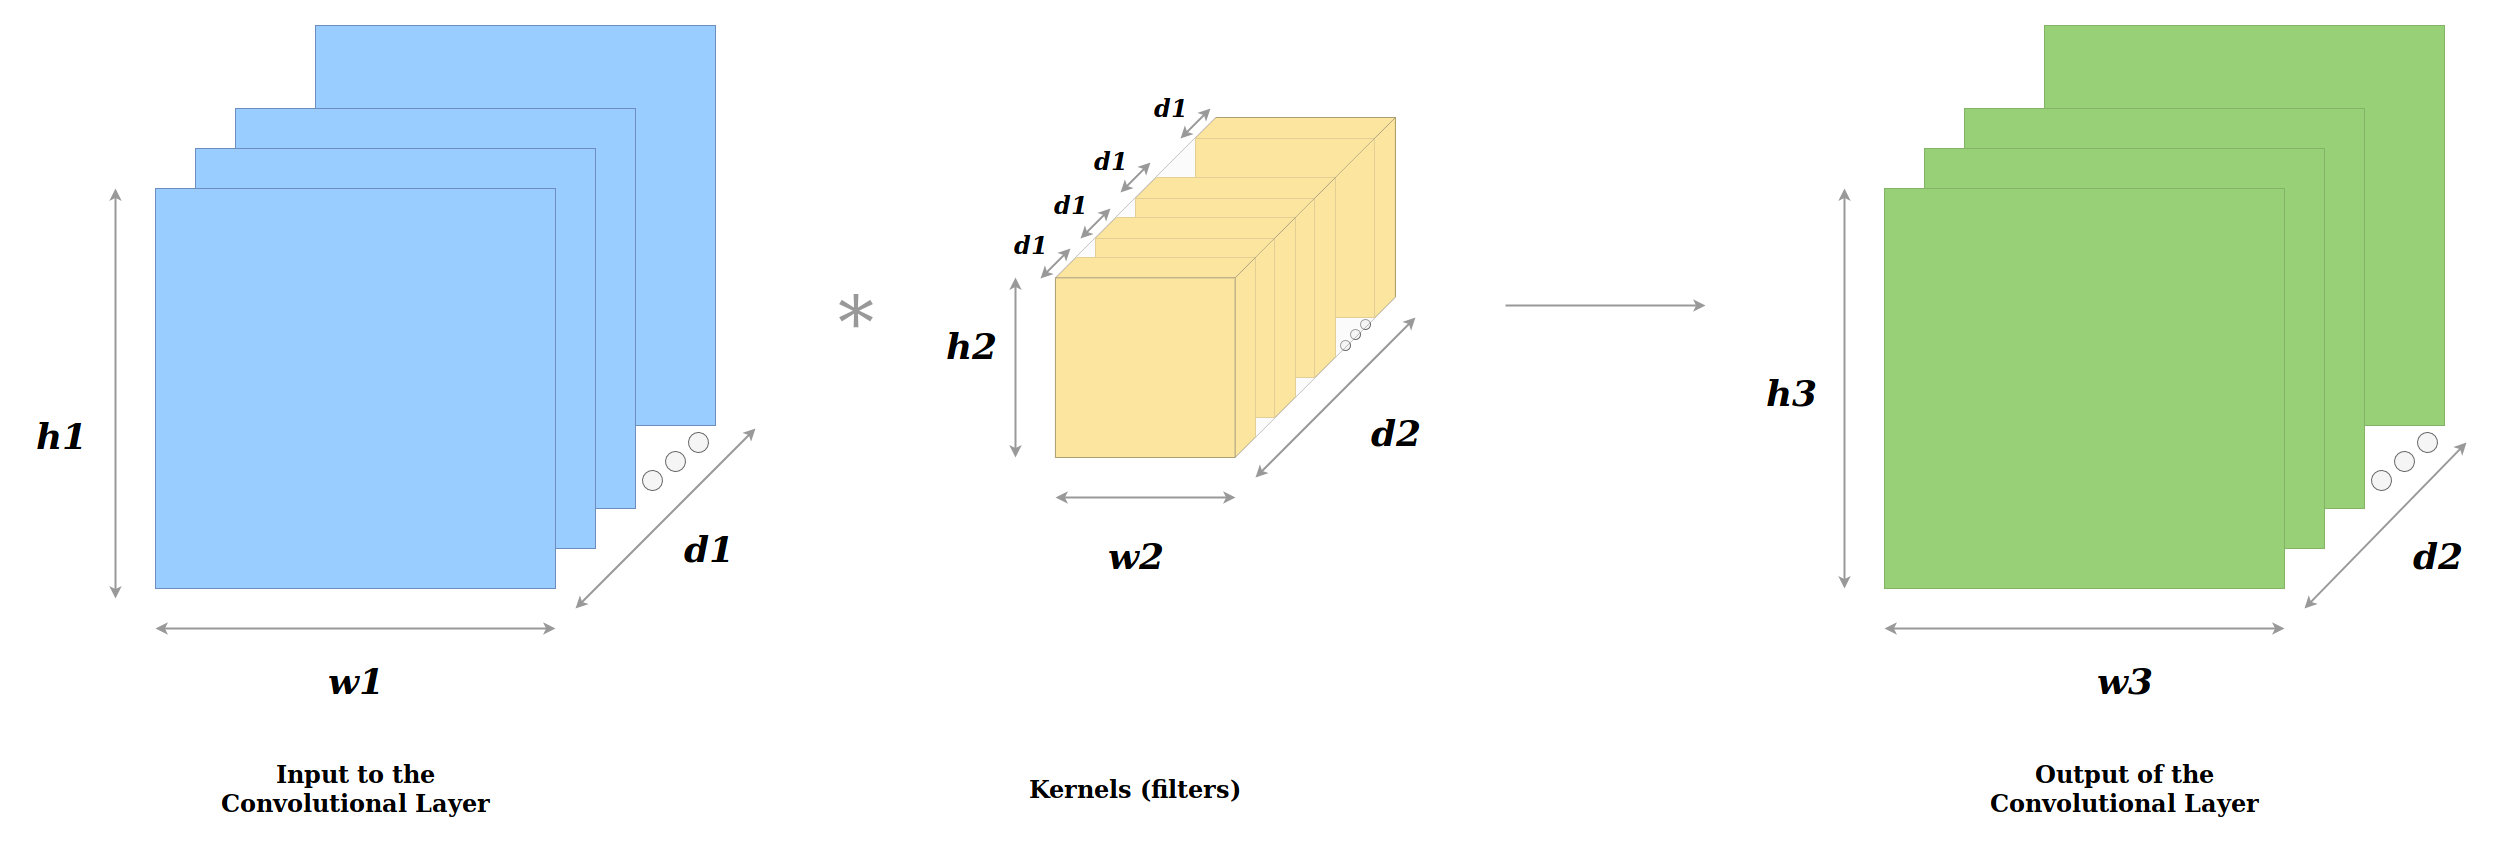
\includegraphics[width=4in]{../cap2_CNNs/src/conv2d.png}
    \caption{\textsc{La convolución 2D puede ser usada con características de $d_1$ canales y devolver una característica de $d_2$ canales.}} 
\end{figure}
 %------------------------------ Padding -----------------------
 \subsection{Padding}
 Debido a que la operación de convolución utiliza  pixeles adyacentes, no es posible calcular los bordes de la imagen resultante. Suponiendo que se tiene una imagen de $n\times n$ y un kernel de $k\times k$ con $k$ impar. Sólo es posible calcular la parte interior de la imagen resultante de tamaño $n-k+1$.
 \begin{figure}[H]
    \centering
     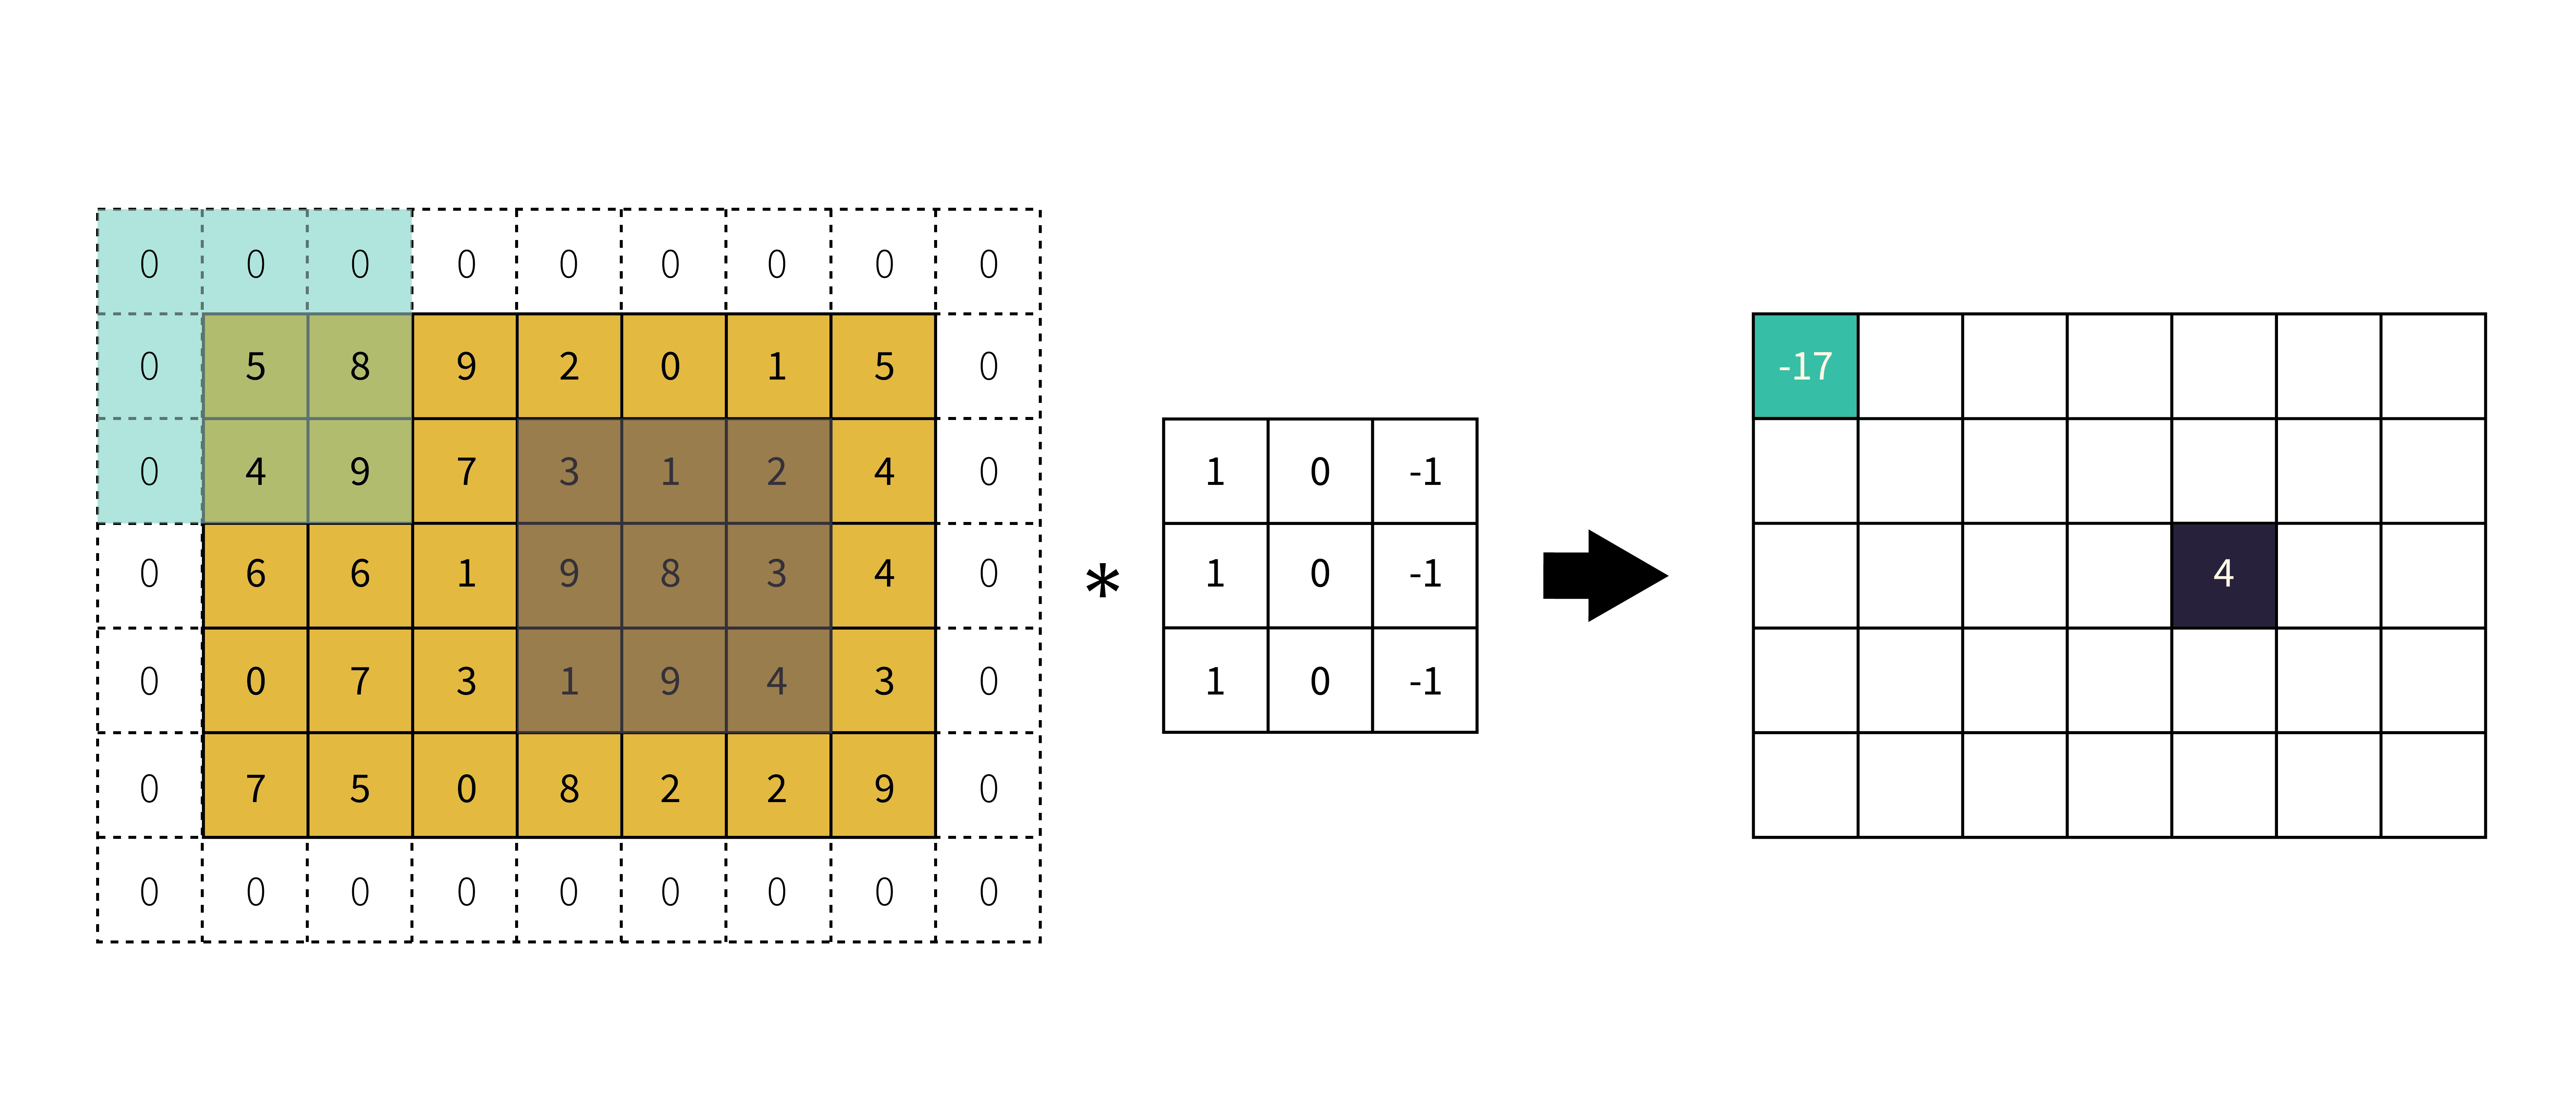
\includegraphics[width = 5in]{../cap2_CNNs/src/padding.png}
     \caption{\textcolor{red}{Usar una imagen propia}}
 \end{figure} 
 Para solucionar este problema, en vez de hacer la convolución con nuestra imagen original $I$, extendemos nuestra imagen hacia todos lados $\frac{k-1}{2}$ pixeles y realizamos nuestra nueva convolución con nuestra imagen extendida $\tilde I$.
 Nuestra nueva imagen $\tilde I$ contiene la misma información que la imagen original $I$, por tanto no importa la información que se añada en los nuevos pixeles. Sin embargo varias estrategias heurísticas han sido desarrolladas con el paso de los años:
\begin{itemize}
    \item \textcolor{red}{\textbf{Constant Padding.}} Cuando  se agrega un valor $c$ en todo el borde. Cuando $c = 0$ se conoce como \textcolor{red}{Zero Padding}.
    \item \textcolor{red}{\textbf{Zero Padding.}} Una posible opción y de las más utilizadas, es agregar ceros en el borde. En \cite{padding} se descubrió que utilizando este tipo de \textcolor{red}{padding} codifica cierto grado de información de las posiciones absolutas. Efecto que no ocurre cuando no se utiliza ningún tipo de \textcolor{red}{padding}. 
    \item \textcolor{red}{\textbf{Reflection Padding.}} Este padding se basa en reflejar los valores con respecto al borde \cite{type_of_paddings}.
    \item \textcolor{red}{\textbf{Symmetric Padding.}} Este padding es muy similar al \textcolor{red}{reflection padding}. En cada fila toma todos los valores y los invierte. Siendo esto lo que aparece en los bordes.
\end{itemize}
\begin{definition}
    Sea $x\in \mathbb R^{h\times w}$ una caracetrística. Sea $\tilde x \in R^{(h+2s)\times (w+2r)}$ con $s < h$ y $r < w$ nuestra caraceterística extendida. Definimos cada \textcolor{red}{padding} como sigue:
    \begin{enumerate}
        \item \textcolor{red}{Zero Padding}: 
        \begin{equation}           
            \tilde x_{i,j} = \left\{ 
                \begin{matrix}
                    x_{i-s, j-r} & \text{si} & s< i <h+s \quad \text{ y } \quad r< j < w+r \\
                    0 & \text{en otro caso}
                \end{matrix}
            \right..
        \end{equation}
        \item \textcolor{red}{Reflection Padding}:
        \begin{equation}           
            \tilde x_{i,j} = \left\{ 
                \begin{matrix}
                    x_{i-s, j-r} & \text{si} & s< i <h+s \quad \text{ y } \quad r< j < w+r \\
                    x_{i-s, r-j+2} & \text{si} & j < r \\
                    x_{s-i+2, j-r} & \text{si} & i < s \\
                    x_{2h+s-i, j-r} & \text{si} & i > h+s \\
                    x_{i-s, 2w+r-j} & \text{si} & j > w+r \\
                \end{matrix}
            \right..
        \end{equation}
        \item \textcolor{red}{Symmetric Padding:}
        \begin{equation}           
            \tilde x_{i,j} = \left\{ 
                \begin{matrix}
                    x_{i-s, j-r} & \text{si} & s< i <h+s \quad \text{ y } \quad r< j < w+r \\
                    x_{i-s, r-j+2} & \text{si} & j < r \\
                    x_{s-i+2, j-r} & \text{si} & i < s \\
                    x_{2h+s-i, j-r} & \text{si} & i > h+s \\
                    x_{i-s, 2w+r-j} & \text{si} & j > w+r \\
                \end{matrix}
            \right..
        \end{equation}
    \end{enumerate}  
\end{definition}
En \cite{type_of_paddings} tras un estudio exhaustivo en el Image Net concluyen que el \textcolor{red}{symmetric padding} y el \textcolor{red}{reflection padding} obtienen peores resultados que el \textcolor{red}{Zero padding}. 
 %------------------------------ Pooling -----------------------
\subsection{\textcolor{red}{Pooling}}
Una vez que nuestra red encuentra características en una imagen, es posible que algunas secciones relevantes sean más grandes que otras. Por eso mismo, se implementa el \textcolor{red}{Downsampling}, es decir reducir el tamaño de nuestras imágenes, para que nuestro kernel pueda encontrar cosas de distintos tamaños conforme nuestras capas van reduciendo el tamaño de la imagen. La pregunta que surge es, ¿Cómo reducimos el tamaño de una imagen?  Sea como sea, siempre algo de información se pierde. Sin embargo existen métodos para resumir la información de varios pixeles en un sólo pixel. Algunos de estos métodos son
\begin{itemize}
    \item \textcolor{red}{\textbf{Max Pooling}}. Dada una vecindad rectangular de pixeles, el \textcolor{red}{maxpooling} consiste en tomar el máximo valor dentro de esta vecindad. 
    \item \textcolor{red}{\textbf{Average Pooling}}. Al igual que en el anterior caso, se toma una vecindad rectangular de pixeles. Sin embargo, en este caso se toma el promedio de todos los pixeles.
    \item \textcolor{red}{\textbf{Una punto intermedio}}. Considérese $v$ el vector de pixeles que debe reducirse a un sólo pixel . En \cite{pooling_analysis} se analiza el uso de diferentes \textcolor{red}{poolings}, y se obtienen distintas parametrizaciones para hallar el valor del pixel $f_P(v)$ que sintetiza la información de $\mathcal v$. Una posible parametrización es $f_P(v) = \left(\frac{1}{N}\sum_{i= 1}^{N}v_i^P\right)^{\frac{1}{P}}$. Donde $P=1$ es el \textcolor{red}{average} y si $P\to \infty$ es el \textcolor{red}{maxpooling}. Por tanto, es posible utilizar otros valores de $P$ para obtener \textcolor{red}{poolings} diferentes.
\end{itemize}
\begin{figure}[H]
    \centering
    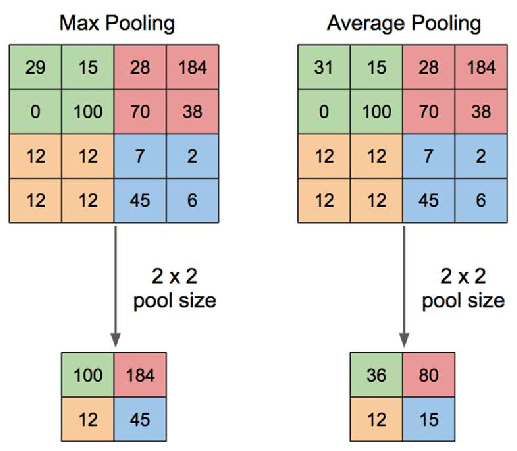
\includegraphics[width=4in]{../cap2_CNNs/src/pooling.png}
    \caption{\textsc{Ejemplo de maxpooling y averagepooling con regiones rectangulares de $2\times 2$.}} 
\end{figure}
También es posible en vez de hacer un \textcolor{red}{pooling} hacer una convolución con cierto tamaño de paso, con la intención de reducir el tamaño de la imagen. Esto no ha remplazado al \textcolor{red}{maxpooling} pero en la literatura se observan resultados prometedores. 
% ------------------------ Global pooling layers
\subsubsection{\textcolor{red}{Global pooling layers} }
Además de hacer un \textcolor{red}{downsampling}, también es común que en algún punto de nuestra red, se reduzca una característica a un valor escalar, o en caso de una imagen con $d$ canales es posible obtener un vector en $\mathbb R^d$ \cite{CNNdefinition}.
\begin{definition}
    Sea $x\in \mathbb R^{h\times w}$ una característica. El operador \textcolor{red}{global average pooling}, $P_g: \mathbb R^{hw}\to \mathbb R$ se define como:
    \begin{equation}
        P_g(x) = \frac{1}{hw}\sum_{i=1}^h\sum_{j=1}^w x_{i,j}.
    \end{equation}
    Más aún, sea $x \in \mathbb R^{h\times w \times d}$ una característica. El operador \textcolor{red}{global average pooling}, $P_g: \mathbb R^{hw}\to \mathbb R$ se define como:
    \begin{equation}
        P_g(x) = (P_g(x_1), ..., P_g(x_d)).
    \end{equation}
\end{definition}
\textcolor{red}{falta aclarar la notación de $x_i$, $x_{i,j}$ y $x_{i,j,k}$}
% ------------------------ Convolución como una operación lineal
\subsection{\textcolor{blue}{Convolución como una operación lineal}}
 Es posible ver una convolución como una multiplicación por una matriz poco densa, en donde varios elementos de la matriz están restringidos a ser iguales a otros. Para las convoluciones de una variable, tienen que ser una \textsl{matriz de toeplitz}. En lo que refiere a dos dimensiones, una convolución es equivalente a una \textsl{Doble Matriz Circulante por Bloques} [Definición \ref{doubly_circulant_matrix}]. Es decir, se tiene lo siguiente 
 \begin{corollary}
    Sea $I$ una imagen, y $K$ un kernel. Existe una matriz $\hat K$ 
    \begin{equation}
        I*K = \text{vec}(I)\hat K.
    \end{equation}
 \end{corollary}
 \textcolor{red}{Falta explicar que las convoluciones son invariantes a las traslaciones.}

 %------------------------------ Redes Neuronales convolucionales -----------------------
\section{Redes Neuronales Convolucionales}
Consideremos el problema de clasificación. Sea $m$ la cantidad de clases posibles. Dados $y_1, y_2, ..., y_s \in \mathbb R^n$ y sus etiquetas $c_1, c_2, ..., c_s\in \mathbb R^m$, en donde la $k$-ésima entrada de $c_i$ \textcolor{blue}{representa la probabilidad de que $y_i$ pertenezca a la clase $k$.}

    Sean 
    \begin{equation}
        \label{clasification}
        Y_0 = [y_1, y_2, ..., y_s]^T \quad \text{ y }, \quad  C = [c_1, ..., c_s]^T.
    \end{equation}

    El objetivo es poder clasificar correctamente datos no etiquetados. Para ello se han desarrollado diferentes arquitecturas de redes neuronales, y en el \textcolor{blue}{2015} las \textsl{Redes Neuronales Convolucionales} obtuvieron el primer lugar en el \textcolor{blue}{Image Net}, consiguiendo resultados sin precedenes. 

 %------------- Descenso del gradiente
\subsection{Descenso del Gradiente Estocástico}
Ya que el problema de aprendizaje, es un problema de optimización, podemos recurrir a la teoría de optimización conocida. El algoritmo más común en el aprenizaje automático es el \textsl{descenso de gradiente estocástico} (SGD por sus siglas en inglés), el cuál es un algoritmo numérico para encontrar mínimos locales de una función. La intuición se basa en que si se tiene un punto $x\in D_f$, la dirección en dónde más decrece es $-\nabla f$. Éste método consiste en dos pasos
\begin{enumerate}
    \item Se selecciona un punto inicial $x_0$ en el dominio.
    \item Se actualiza nuestro valor $x_{i+1} = x_i - \alpha\nabla f(x_i)$ para $i = 1, ... N$
\end{enumerate}
donde $N$ es el número de iteraciones totales y $\alpha$ es un escalar, el cuál se conoce como ratio de aprendizaje (learning rate). Es importante seleccionar un ratio de aprendizaje apropiado, pues en caso de seleccionar uno muy grande, el algoritmo podría diverger, por el contrario si se selecciona uno muy pequeño, entonces el entrenamiento podría ser demasiado lento. 

Para calcular el gradiente de manera exacta, es necesario utilizar todo el conjunto de datos, lo cuál puede traducirse a tiempos elevados de cómputo. Es por eso, que en la práctica, se utiliza únicamente un subconjunto aleatorio de datos, calculando así, una aproximación al gradiente $\nabla J$ de nuestra funcion de costo. Debido a este artificio que reduce el tiempo de entrenamiento, es que nuestro algoritmo es considerado estocástico.
\begin{figure}[H]
    \centering
    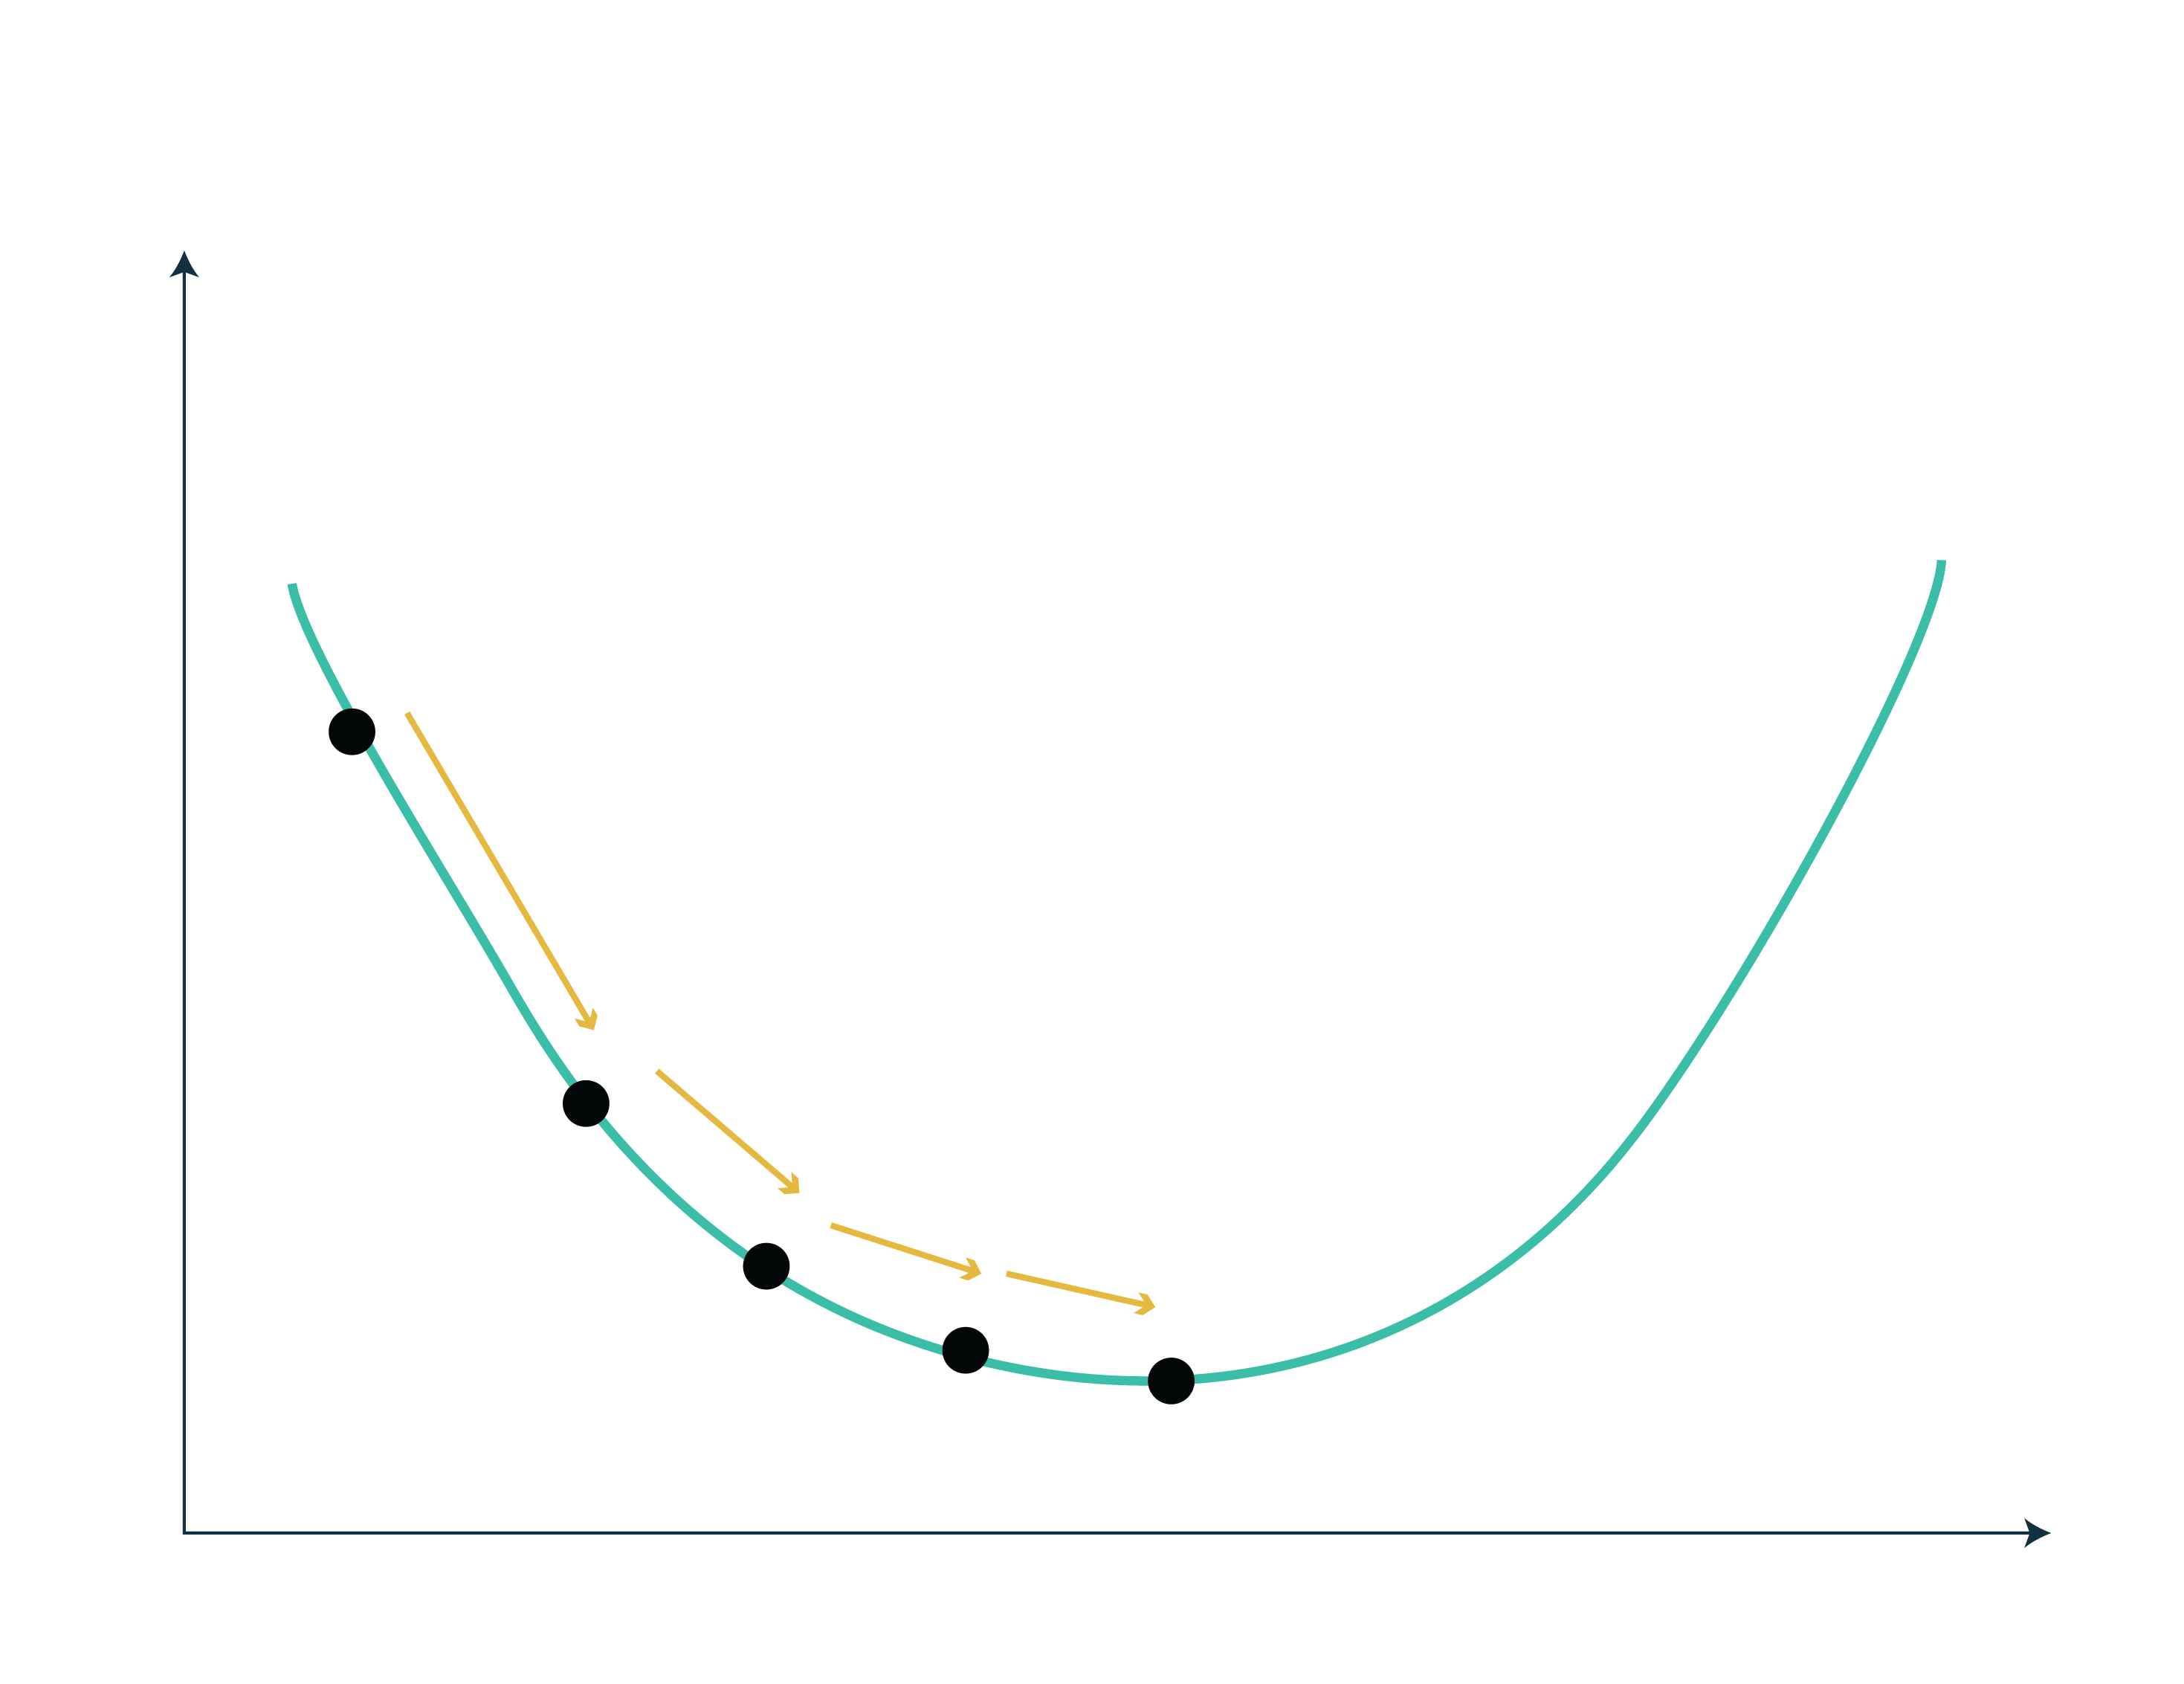
\includegraphics[width=4in]{../cap2_CNNs/src/sgd.png}
    \caption{\textcolor{red}{Seleccionar su propia imagen}} 
\end{figure}
\subsection{Propagación hacia atrás}
Ahora que se tiene un algoritmo para optimizar nuestra función de costo, la pregunta natural es ¿Cómo obtenemos el gradiente? Siendo la propagación hacia adelante de una red, una función tan complicada y con tantos parámetros, es muy difícil calcular de manera analítica nuestro gradiente. Por buena suerte para nosotros, existe una técnica conocida como \textsl{propagación hacia atrás}, encargada de calcular numéricamente el gradiente de la función de costo.


\subsection{Normalización por Lotes}
Entre las téncicas de regularización más utilizadas se encuentra la \textsl{normalización por lotes} (BN por sus siglas en inglés). En el 2015 en un paper de google \cite{batchNormalization} se describe esta técnica y se constata que tiene múltiples beneficios tales como incrementarl el \textcolor{red}{learning rate}, conseguir que el entrenamiento sea más independiente de la inicialización y además actuar como regularizador.

\begin{definition}
    Sea $\mathcal{B} = \{x^{(1)}, x^{(2)}, \ddots, x^{(m)}\}$ un lote de características. La normalización por lotes de $\mathcal B$ se define como:
    \begin{equation}
        B(x^{(i)}; \gamma, \beta) := \frac{\gamma(x^{(i) - \mu})}{\sigma} + \beta, \quad i=1,2...,m,
    \end{equation}
    donde  $\mu := \sum^m_{i=1}x^{(i)}/m$ y $\sigma^2 = \sum^m_{i=1}(x^{(i)}-\mu)^2/m$.
\end{definition}
Los parámetros $\gamma$ y $\beta$ usualmente se aprenden en la optimización. Cuando se usa la normalización por lotes, no es necesario agregar \textcolor{red}{biases} pues son calculados explícitamente a través de $\beta$.

\textcolor{red}{Aquí va la justificación de por qué usar convoluciones}   
\begin{definition} 
    Consideremos el problema de clasificación (\ref{clasification}). La propagación hacia adelante de una CNN está determinada por el siguiente esquema recursivo

    \begin{equation}
        Y_{i+1} = \sigma(Y_i * K_i + b_i).
    \end{equation}
    donde $\sigma$ es una función de activación, $K_i$ representa un Kernel y $b_i\in \mathbb R^n$ es el \textcolor{blue}{bias}.
\end{definition}

\textcolor{red}{Imagen de una Lee Net o AlexNet para entender una arquitectura simple}.


\subsection{Desvanecimiento del gradiente}

\subsection{CNNs en el estado del arte}
En 2012 en el ImageNet ocurrió algo sin precedentes en dicha competencia. El ganador del concurso se había llevado el primer lugar absoluto, obteniendo una ventaja de 10.9$\%$ de error por debajo del segundo lugar. Es así como la \textsl{AlexNet} \cite{alexnet} consiguió reputación para las CNNs. Para 2013, la red ganadora del ImageNet(2013) fue la Zf-net \cite{zfnet}, la cuál era una modificación de los hiperparámetros de la AlexNet.

\begin{figure}[H]
    \centering
    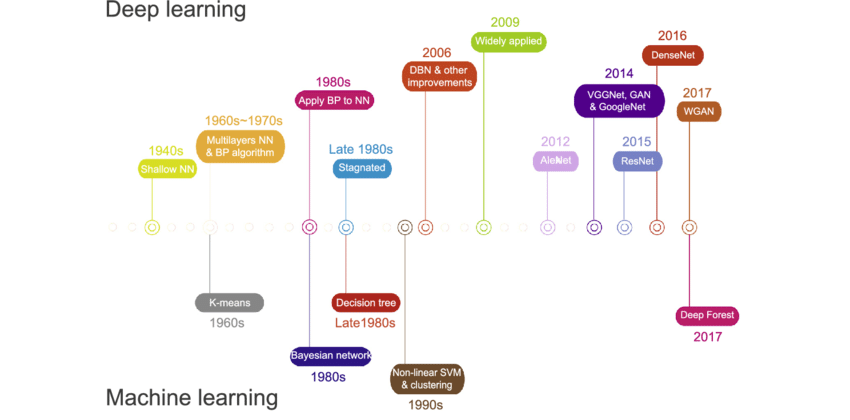
\includegraphics[width=4in]{../cap2_CNNs/src/timeline.png}
    \caption{\textcolor{red}{Crear imagen propia}} 
\end{figure}
 %------------------------------ ResNet -----------------------
\section{ResNet}
Las \textsl{Redes Neuronales Residuales} fueron presentadas en 2015 por Kaiming He \textcolor{blue}{et. al.} en \cite{resnet0}. Uno de los mayores retos en el diseño de redes profundas, es el \textsl{desvanecimiento del gradiente}. Es decir, por la naturaleza del \textcolor{blue}{backpropagation}, las redes muy profundas, implican el cálculo de gradientes con entradas muy pequeñas, y debido a las limitaciones del aritmética de punto flotante, ésto provoca que el gradiente se desvanezca.
Es decir, $\|\nabla_\theta L\| = 0$ dónde $L$ es la función de pérdida y $\theta$ son los parámetros. 

Antes del 2015 existían dificultades para alcanzar redes con profundidades mayores a 20 capas. Para solucionar este problema, se crearon las \textsl{conexiones de salto}.

\begin{definition} 
    Consideremos el problema de clasificación (\ref{clasification}). La propagación hacia adelante de la ResNet está determinada por el siguiente esquema recursivo

    \begin{equation}
        Y_{i+1} = Y_i + \sigma(Y_i * K_i + b_i).
    \end{equation}
    donde $\sigma$ es una función de activación, $K_i$ representa un Kernel y $b_i\in \mathbb R^n$ es el \textcolor{blue}{bias}.
\end{definition}
Ya que las matrices 
 %------------- Estabilidad de las redes neuronales
\subsection{Estabilidad en las redes Neuronales}
En clasificación de imágenes, una red debe ser robusta contra el ruido, o pequeñas modificaciones en la imagen. \textcolor{red}{La salida debe ser continua con respecto a la entrada}.

\begin{definition}
    Supóngase $f$ la propagación hacia adelante de una red neuronal. Sea $x$ una imagen y $\hat x$ la misma imagen perturbada. Decimos que $f$ es estable cuando 
    \begin{equation}
        \|f(x)-f(\hat x)\| < \epsilon
    \end{equation}
    donde \textcolor{red}{epsilon es muy pequeño}
\end{definition}
En \cite{stable_resnets} se agrega un término $h\in \mathbb R$ a la ResNet con la intención de añadirle estabilidad a la red
\begin{equation}
    Y_{i+1} = Y_i + h\sigma(Y_iK_i + b_i).
\end{equation}
 %------------- Notas del capítulo
 \section{Notas del capítulo}
 \begin{enumerate}
     \item Añadir la definición de stride en la sección de convoluciones
     \item El capítulo de ResNet podría llamarse Redes Neuronales convolucionales
     \item No estoy seguro de si dedicarle un capítulo completo al desvanecimiento de gradiente, o sólo mencionarlo en el capítulo de ResNets. Por lo pronto, lo menciono en el capítulo  de resNets
     \item Debo mencionar lo que significa el gradiente en los preliminares
     \item Cuando definimos el problema de clasificación, decimos que $y_i\in \mathbb R^n$. Me gustaría que pudiese hablar de $y_i$ como imágenes, es decir $y_i\in \mathbb R{n_1\times n_2 \times d}$. 
     \item En preliminares falta escribir un poco de visión computacional. ¿Qué es una imagen? ¿Qué significa perturbar una imagen o meterle ruido?
     \item Traducir Batch Normalization
     \item Aún falta definir matemáticamente el symmetric padding
 \end{enumerate}

 % \begin{definition}
 %     Sea $x$ una característica en $\mathbb R^{h\times w}$ y $K$ un filtro de $(2r + 1) \times (2r+1)$. La \textsl{convolución por canal} de $x$ y $K$, a la cual denotaremos $y:= K \bigotimes x$, es una característica en $\R ^{h \times w}$ tal que:
 %     \begin{equation}
 %         y_{i,j} :=  \sum_{l,k=-r}^r K_{l+r+1, k+r+1} x_{i+l, j+k} 
 %     \end{equation}
 %     para todo $i = 1,2,..., h$ y $j = 1,2,..., w$.
 % \end{definition}

 % Es posible extender esta definición para, filtros de $2r\times 2r$, sin embargo, los tamaños más comunes de kernels son $3\times 3$ y $5\times 5$.
 